\subsection{Setup procedures}
    \subsubsection{Neural network architecture}
        As was described in section \ref{subsection:dl} the choice of the model architecture fell onto the UNet. Here will be provided a detailed decription of the architecture and the different layers used. An architecture used in this research was chosen based on paper [TODO LaChance]. The input to this network is a $256 \times 256$-pixel DIC image that should be already preprocessed with the corresponding to the desired organelle preprocessing pipeline. Specifications about different preprocessings are described separately in the separate subsections of different organelles.

The encoder part of the UNet (Figure \ref{fig:unet}) step by step compresses spatial dimensions of the image (the spatial dimension size is detoned by a number on the left of each green block) into tensors or feature maps with an increasing amount of filters (filters are denoted by a number on the top of each green block). This allows to reduce the spatial information in the image and capture semantics. Decoder part on the contrary decompresses feature maps gradually increasing the amount of spatial information in tensors and reducing the number of filters. All convolutional layers use convolution of size $3 \times 3$ with the corresponding number of filters that are denoted in the Figure. Downsapling in encoder reduces the spatial dimension twice during each step and implemented using max-pooling with a size of $2 \times 2$. Upsampling in decoder increases the spatial dimension also twice during each step and implemented using transposed convolution with a size of $2 \times 2$. After the first convolution layer after each max-pooling step a batch normalization layer was used as they are well-known for speeding up the training process [cite Ioffe]. One should not forget though that using batch normalization might be sometimes dangerous due to the leak of information [cite Fetterman 2020]. Additionally dropouts were used for example for actin predictions as the model would encounter overfit quite easily there, however for default choice dropouts were not pressent. That is another thing that differs this architecture from the original in [TODO Cite LaChance] paper. The last layer of the UNet is a sigmoid activation function.
\begin{figure}[htb]
	\begin{center}
		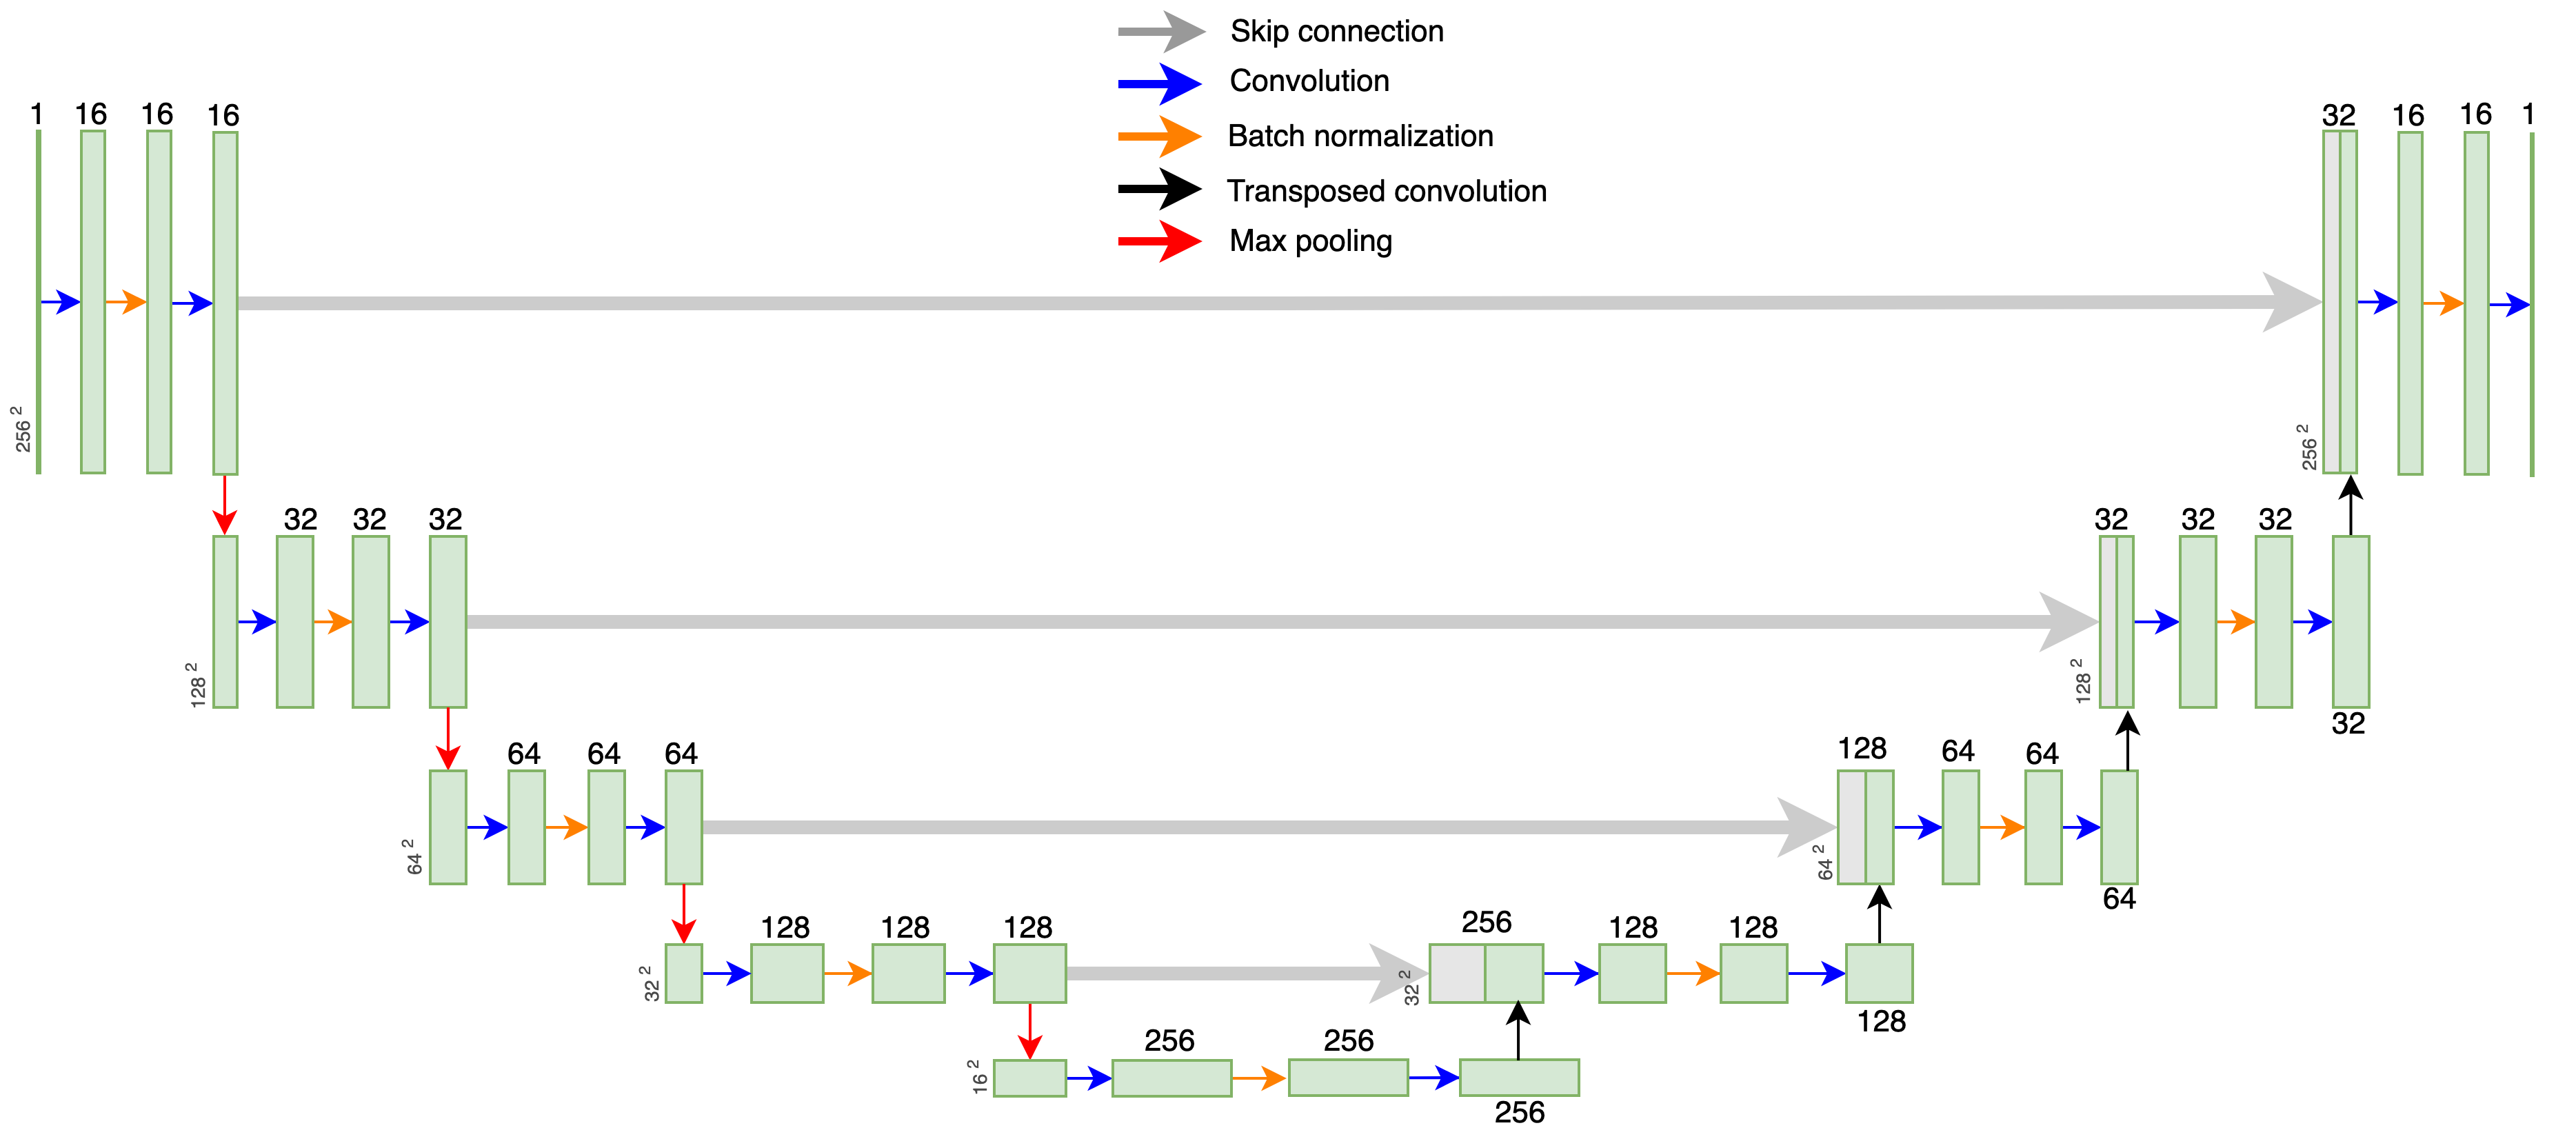
\includegraphics[width=\linewidth]{bilder/Unet.png}
		\caption{Unet}\label{fig:unet}
	\end{center}
\end{figure}

There is a space for potential improvements regarding the model architecture here: for example, [Shiyui 2021] recommends to use special dense-block after each convolutional layer that would consist of another 3 convolutional layers with 24 filters, Batch normalization layer and ReLU activations each. This could potentially facilitate efficient training of the model, still most probably the efficience comes mostly from Batch normalization layers that are already used in our architecture. Nethertheless the idea of using the bigger model as [Shiyui 2021], more specifically using more filters, indeed improves the predictions as it will be explained in Section [TODO ref section]. That leaves the plave available for further research and improvements regarding the size of the model and the additionally used dense-blocks. 

An interesting question that automatically rises here is what do embeddings (output tensors from the encoder) represent. There is a big difference between any representation learning network such as an autoencoder and a UNet - a UNet model uses skip-connections that allow to propagate an information between its encoder and a decoder. Meaning that embeddings do not contain purely semantic information, because essentially the network is not pushed to compress the information severely (as autoencoder would do), but it should only to extract relevant for segmentation features. One of the questions solved in this work was wether or not UNet embeddings are clustering based on the following classes: cell phenotypes, any kind of corruption within the data. For example, it would be bery usefull to be able to not only predict the data itselt, but also to say wethere the prediction is reliable of not. The initial hypothesis here would be that if the predictions are not of a good enough quality this would also be reflected in the embeddings. 
    \subsubsection{Available data}
        Description of the datasets and the amount of images in each category.

\begin{table}[H]
    \centering
    \caption{Available data for each fo the organelles}
        \begin{adjustbox}{width=0.7\textwidth}
            \begin{tabular}{|c||c|c|c|c|}\hline
                &Total images
                &Training crops
                &Validation crops
                &Test crops
                \\\hline\hline
                Nuclei &595&27,264&3,008&7,616\\\hline
                Actin &400&18,432&2,048&5120\\\hline
                Golgi &761&23,036&2,336&6,347\\\hline
                H19 &400&27,264&3,008&7,61\\\hline
                Nucleolei &?&?&?&?\\\hline
            \end{tabular}
        \end{adjustbox}
\end{table}

    \subsubsection{Training costs estimation}
        For training purposes in this research cloud computing services were used, or more specifically - Amazon Web Services (AWS). These remotely located servers provide an possibility to train your models on a variety of graphic cards paying for minute rate. In order to keep the costs unter the control it was important to estimate the time needed for training in advance to choose the most efficient GPU possible.

Cost estimation is additionally important for the model inference as well during the production. Although for production purposes the lambda functions from AWS can used, then are triggered only when the inference request arrives and are turned off automatically shortly after.

For both training an inference purposes two GPU models were tested g3-4xlarge which is an NVIDIA Tesla M60 and p3-2xlarge which is a NVIDIA Tesla V100. The datasets on which the experiments were performed on were a nuclei training and validation dataset. The resulting costs are presented in the Tables \ref{table:costs-training}, \ref{table:costs-inference}.

\begin{table}[H]
    \centering
    \caption{Costs estimations of AWS use for training models}
        \begin{adjustbox}{width=0.7\textwidth}
            \begin{tabular}{|c||c|c|c|c|}\hline
                &Runtime (1 epoch)
                &Dataset size
                &Costs per minute
                &Cost per epoch
                \\\hline\hline
                g3.4xlarge & $6.5 mins$ & $18,432$ & $0.07125\$$ & $0.3$\\\hline
                p3.2xlarge & $400$ & $18,432$ & $0.1911\$$ &$0.18$\\\hline
            \end{tabular}
        \end{adjustbox}
    \label{table:costs-training}
\end{table}

%g3 391, 261, 260
%p3 170, 57, 56


\begin{table}[H]
    \centering
    \caption{Costs estimations of AWS use for inference purposes}
        \begin{adjustbox}{width=0.7\textwidth}
            \begin{tabular}{|c||c|c|c|c|}\hline
                &Runtime
                &Dataset size
                &Costs per minute
                &Cost of inference
                \\\hline\hline
                g3.4xlarge & $?\text{mins}$ & $2,048$ & $0.07125$ & $? \$$\\\hline
                p3.2xlarge & $?\text{mins}$ &  $2,048$ & $0.1911$ &$? \$$\\\hline
            \end{tabular}
        \end{adjustbox}
    \label{table:costs-inference}
\end{table}

As a conclusion even though a p3 instance seems to be much more expensive, it is also much more efficient and the costs estimated to training times are lower. That is why all the training experiments in this research were conducted on an NVIDIA Tesla V100 GPU.
    \subsubsection{Augmentations}
        \label{section:augmentations}
        Augmentations are a powerful regularization technique that helps the network to generalize better [cite Wang 2017] and is an effective solution for a situation with the lack of labeled data [cite Yang 2022]. The main idea behind augmentation is to increase the diversity of training data, when the acquisition of the real training data is expensive. Augmenting existing images creates the new synthetic samples which are hypothetically very close to the original true distribution of images. However, one should be very cautios regarding the type of augmentations that can be used. Augmentation must enrich the dataset, but it should not change the semantics hidden in each image. The peculiarity of current research is the pair-wise correspondence between the DIC input and the output fluorescence. One should not change the input in such a way that the fluorescence signal could not be inferred from it. Therefore the following augmentations have been used on cropped images:

\begin{itemize}
	\item \textbf{Flipping}: Flip the crop horizontally (30\% chance), vertically (30\% chance) or both.
	\item \textbf{Random rotation}: Rotates the crop by a random angle.
	\item \textbf{Random scaling}: Reduces crop size by 100 (20\% chance), 50 (20\% chance) or 20 (60\% chance) pixels from each side (down, top, left, right).
	\item \textbf{Contrast}: Halves an image's constrast (50\% chance), or triples it (50\% chance). Applied with a 20\% chance.
	\item \textbf{Defocus blur}: Imitates a defocus blur of severity level 4 (see section [TODO cite section]) on an image with a 20\% chance.
\end{itemize}

\paragraph{Special augmentations for rotation and scaling}

Augmentations are chosen to be applied during training and the reason for that is to preserve the same conditions regarding the size of the datasets in order to have a fair comparison between approaches. For example, one decides to augment 20\% of images and add them to an original dataset in order to expand it. Then the comparison between training with and without augmentations would be unfair as the sizes of the datasets are different, and it is not clear whether the performance improvement or decrease comes from the longer training (enlarged dataset) or augmentations.

Since augmentations are applied on crops directly during training there is a possibility to improve the rotation and scale of crops. The problem with these augmentations are depicted in Figure \ref{fig:smart-augments} - after applying them the a gray background will appear which would be filled with zeros in PyToch implementation. However, since an original image where the crop has been cut out is available, one can easily restore the background with the original values and avoid this problem entirely.

\begin{figure}[H]
	\begin{center}
		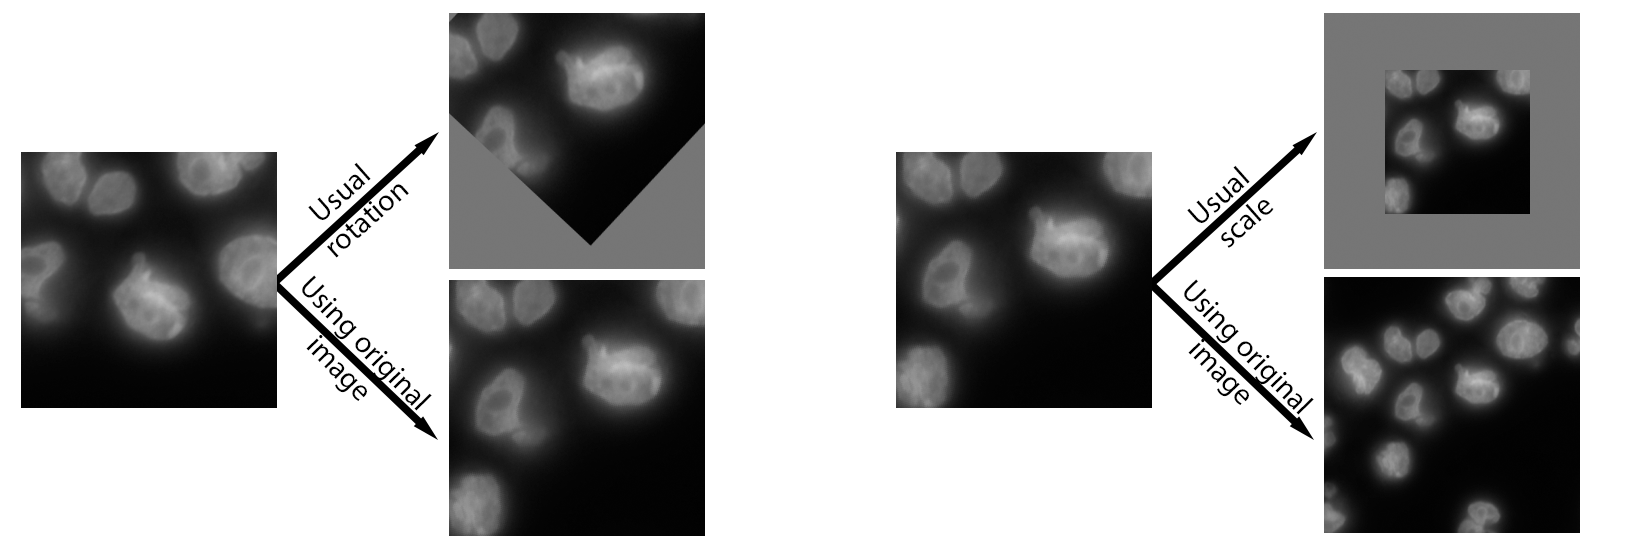
\includegraphics[width=0.7\linewidth]{bilder/model training/smart augmentations.png}
		\caption{Using original image for rotation and scaling augmentations}\label{fig:smart-augments}
	\end{center}
\end{figure}

Applying augmentations in combination with other regularization techniques has proven to be helpful against overfitting for the nuclei and ER training. Therefore it is recommended to use it in further research as well.

    \subsubsection{Model setup}
        \paragraph{Weight initialization}
            In order to achieve best predictions results it is very important to pre-setup a model correctly. Since the architecture used here is very similar to the one used in LaChance paper, the setup configuration is similar as well.  
            Weight initialization plays a crucial role in model training. Even on the simplest model wrongly initialized weights (for example all constant or too large or too small) can lead to very slow convergence or prevent the model from converging at all (\cite{Kumar_2017}).

Xavier initialization, which is usually a default choice in many neural networks, works well for the most part for fully connected layers with tanh as activation function. There is also a study providing some insights into why Xavier initialization may not be the optimal choice for ReLU activations (\cite{Kumar_2017}). In the following samples \textit{fan\_in} denotes the maximum number of input signal units to a given layer and \textit{fan\_out} is the maximum number of output signal units from it. A definition of Xavier initialization can be found below:

Research of \cite{He_2015} also notices the problems with Xavier initialization for ReLU activations. The authors suggest a new robust method called He initialization that enables training of even extremely deep or wide network architectures with ReLU activations. This method was suggested by the \cite{Lachance_2020} paper and has been used in this reseach as well. He initialization draws samples from a truncated normal distribution:
\begin{equation}
	N(0, \sqrt{\frac{2}{\text{fan\_in}}})
\end{equation}

Default weight initialization of Conv2D layers in Python claims to uses the following initialization method the initialization method (\cite{He_2015}):
\begin{align}
	std &= \sqrt{\frac{2}{fan\_in}} \\
	bou&nd = \sqrt{3 * std} \\
	Un&iform(-bound, bound)
\end{align}

Altough in the study of \cite{He_2015} it is called Kaiming normal initialization it is not exactly it. However, the naming is quite confusing and therefore two experiments have been conducted: first, the model predicting nuclei target was trained with the default weight initialization provided by PyTorch and then the initialization was switched to a true He initialization.

\begin{figure}[H]
	\begin{center}
		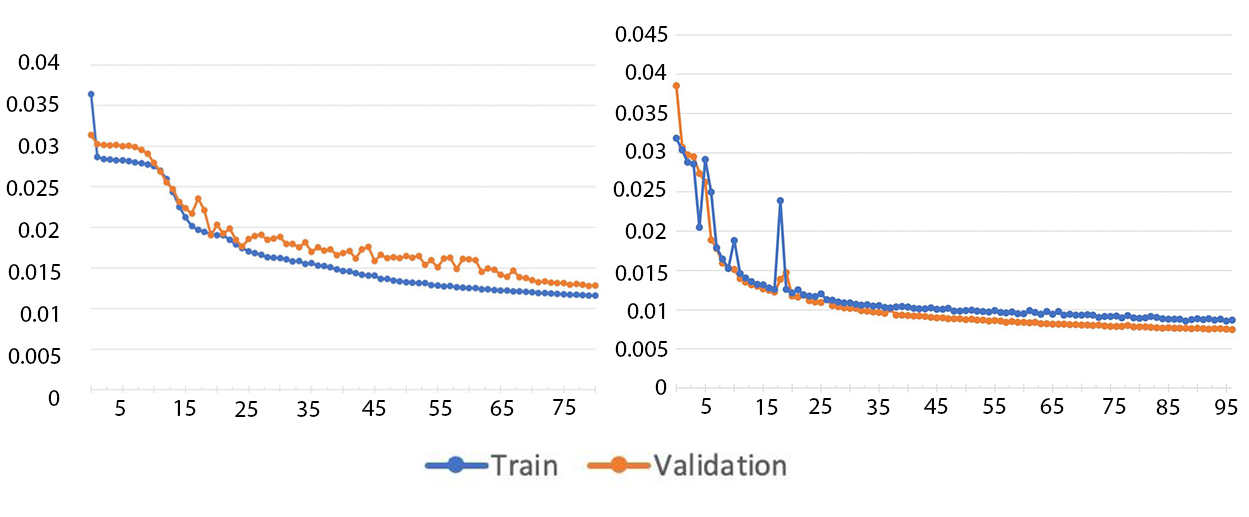
\includegraphics[width=0.8\linewidth]{bilder/nuclei/wi-no-wi.png}
		\caption[Nuclei training without (left) and with (right) custom weight initialization]%
		{Nuclei training without (left) and with (right) custom weight initialization. The stagnation during first few epochs on the left signalizes about the wrong initialization of model's weights. As a result the left model also converges to a higher value.}\label{fig:wi}
	\end{center}
\end{figure}

The results of the experiments are presented in Figure \ref{fig:wi}. As can be seen, the loss in the left plots stagnates during the first few epochs and then begins to converge later. This is a symptom of a wrong initialization of the weights. Even after the convergence begins, the model still has a higher loss than the one on the right (around 0.012 in comparison to 0.007). However, the model on the right is not completely perfect as the loss still does not converge at the same speed everywhere. Although this might be not related to the weight initialization but more the to instability of the training in general as there were only few images used for these experiments.

        \paragraph{Regularization}
            \label{section:regularization}
            % TODO add overfitting image?
Regularization is mostly used to prevent a deep learning model to overfitting on the training data and to be able to generalize well. Overfitting has occured in the models used in this research and therefore it is improtant to understand the techniques that can be used to prevent it. There are are several approaches to regularize the model and they will be explained below.

\begin{itemize}
	\item Early-stopping

	Overfitting can be detected via visualizing train and validation losses. Training behaviour at first will be the usual one, meaning that both train and validation losses are gradually decreasing, however at some point the train loss continues to decrease, whereas the validation loss suddenly starts to increase (see Figure \ref{fig:er-overfit}). Since the model has not seen any of the data from the validation set, it means that it loses its ability to generalize on unseen data, while improving its perfomance on the seen data (train set). This does not happen during earlier epochs. Assuming that the model learns a complex decision surface while training, the weights of the model will be quite small and random with the correct weight initialization and therefore the best decision surface during the early epochs would be a smooth one. But during the later ones the difference in values of the weights grows and they become dissimilar which also means that the decision surface becomes more complex and the model is now able to fit not only the training data itself, but also its noise (\cite{mitchell_1997} p.111). And that is why stopping before the model becomes too complex, meaning to stop before the overfitting point, mitigates this problem.

	\item \emph{L1}- \emph{L2}-regularization

	The complexity of the deep model grows with the number of features it uses, sometimes the model may pay attention to the features that are not important to the outcome, or even considers noise to be a feature. To prevent this one should decrease the weights associated with useless features, however one cannot know ahead of time which of them should be ignored, therefore one may limit them all (\cite{Ying_2019}). In order to do that, a penalty term is added to the loss function:

	\begin{equation}
	\tilde{L}(Y, M(X, \theta)) = L(Y, M(X, \theta)) + \lambda R(\theta)
	\end{equation}

	for some $\lambda > 0$. This is called a \emph{soft-constraint} optimization. When $R(\theta)$ is of the form $R(\theta) = ||\theta||^2_2 = \sqrt{\sum\limits_i \theta_i^2}$ this is called \emph{L2}-regularization. When it is of form $R(\theta) = ||\theta||_1 = \sum\limits_i |\theta_i|$ this is called \emph{L1}-regularization. \emph{L2}-regularization used in combination with backpropagation is equivalent to weight decay. Weight decay is defined by \cite{Hanson_1988} as follows:
	\begin{equation}
		\theta_{t+1} = (1 - \lambda)\theta_t - \alpha \frac{\partial L}{\partial \theta_t}
	\end{equation}

	where $\alpha$ is a learning rate. Weight decay successfully has more effect on the weights along which the gradient change is smaller \cite{Goodfellow_2016}. \emph{L1}-regularization induces sparsity of the weights by assigning some of them to zero, this could also be considered as a feature selection approach.

	\item Regularization layers

	Batch normalization and dropout layers are also considered to be a form of regularization.

	\item Network reduction

	Since learning a too complex and noise-fitting decision surface might be a frequent cause of an overfit, another way to mitigate this would to be reduce the space of the possible decision surfaces and therefore make the surface simpler so that it cannot fit into the noise from the data. By changing the number of adaptive parameters in the network, the complexity can be varied (\cite{Bishop_2006} p.332).

	\item Expansion of the training data

	For a successful training a model needs to have a sufficient amount of quality samples. An expanded dataset can improve the quality of the predictions \cite{Ying_2019}, however only when the model has already performed well on the initial dataset. If the model was performing badly initially, adding more data will not solve the problem. Here having $27,264$ crops of data the model was trained on $5,376$ crops only (two 96-well plates) to find the best structure and regularization first, afterwards the model was retrained using more data and the PCC loss improves from $0.77$, to $0.93$.
\end{itemize}

        \paragraph{Optimizers}
            It is also important to choose a correct optimizer in order for a model to converge as fast as possible. Here, three different optimizers have been tried out --- namely, SGD, Adam and Adadelta optimizers. As a result, the SGD optimizer performed the worst, while Adam and Adadelta optimizer performed similarly with Adadelta converging to slightly better values in the end. Adam optimizer has required some fine-tuning of the learning rate from 0.001 to 0.0001 to achieve the best result. Both Adadelta and Adam can be used for model optimization in this dataset. The experiments were conducted on the truncated dataset of nuclei images using PCC loss.

\begin{figure}[H]
	\begin{center}
		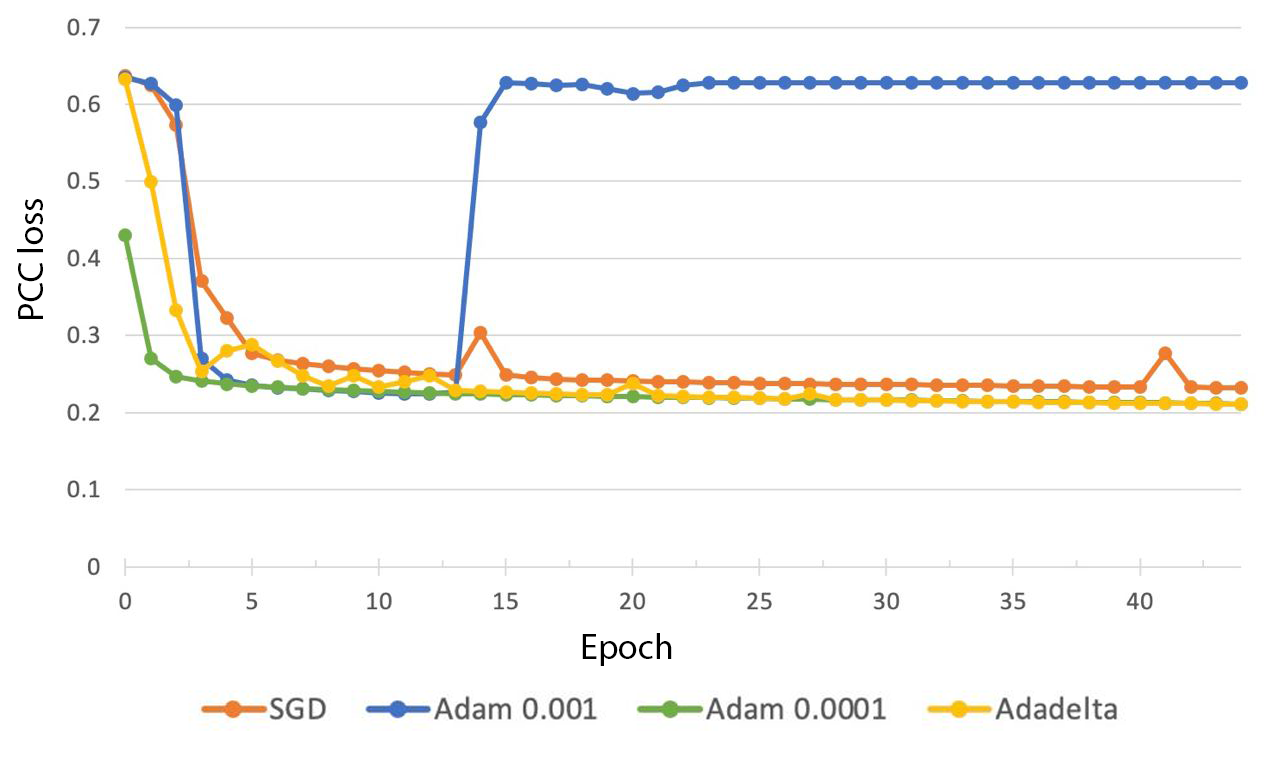
\includegraphics[width=0.8\linewidth]{bilder/model training/optimizer-comparison.png}
		\caption{Comparison of convergence for different optimizers}\label{fig:optimizers}
	\end{center}
\end{figure}

    \subsubsection{Model evaluation: metrics for downstream tasks}
        \label{section:model-evaluation}
        \begin{figure}[H]
	\begin{center}
		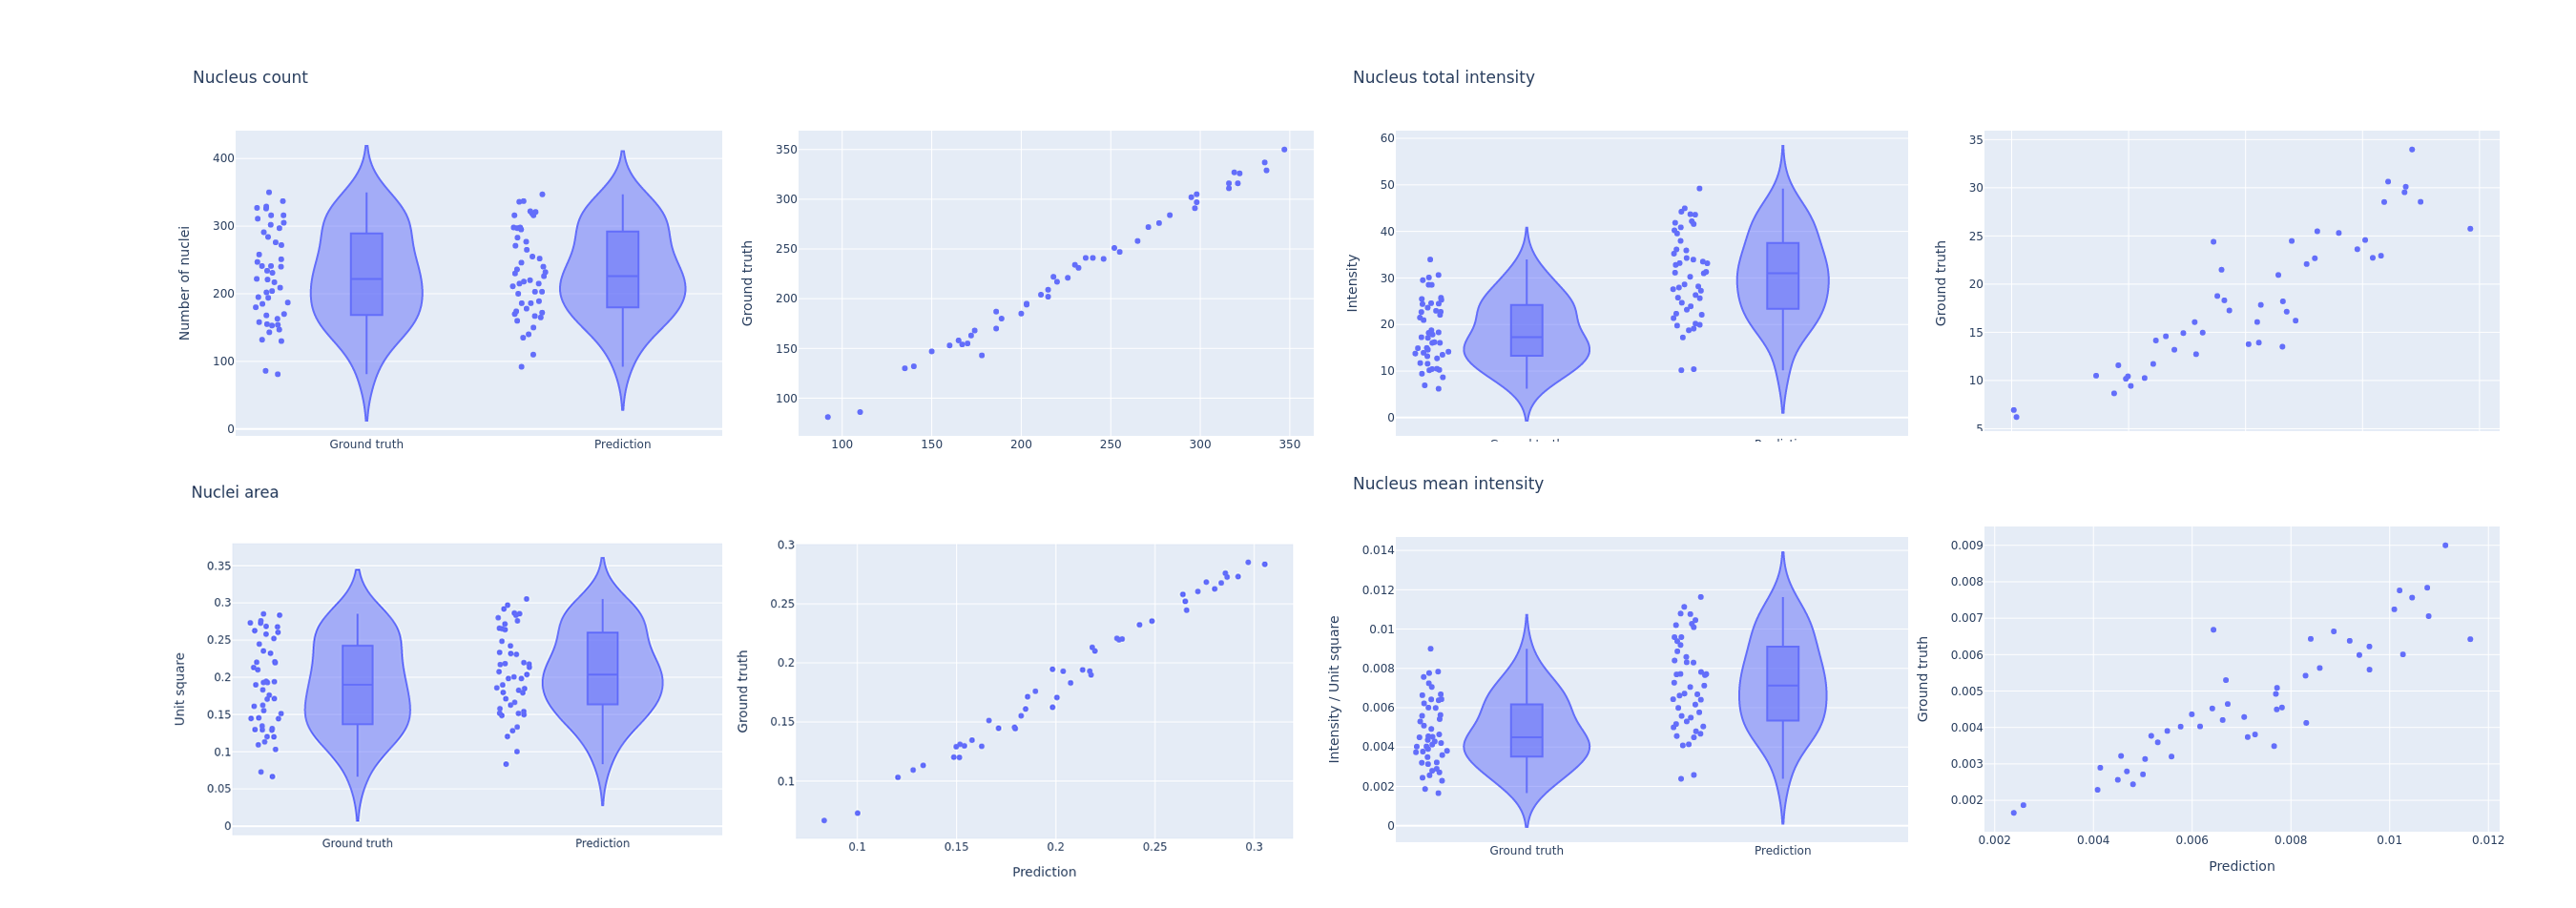
\includegraphics[width=\linewidth]{bilder/nuclei/metric/combined-metrics.png}
		\caption{Metrics for downstream tasks on nuclei}\label{fig:nuclei-downstream-metrics}
	\end{center}
\end{figure}

\begin{table}[H]
    \centering
    \caption{Correlation coefficients for downstream tasks}
        \begin{adjustbox}{width=0.4\textwidth}
            \begin{tabular}{|c|c|c|}\hline
                &Pearson&Spearman
                \\\hline\hline
                Number of nuclei&0.995&0.994\\\hline
                Total intensity&0.902&.911\\\hline
                Mean intensity&0.907&0.904\\\hline
                Area&0.992&0.990\\\hline
            \end{tabular}
        \end{adjustbox}
\end{table}

    \subsubsection{Crops combination technique}\label{par:crops-combination}
        Due to the restricted amount of memory on the GPU deep learning models cannot have a high-resolution image as their input in the scope of this research. Yet this is also not obligatory: as the image contains dozens of cells within it, its processing can be limited to a crop of a smaller size. After the model has predicted fluorescence signal for each of the crops, output fluorescence images can be combined together to form a high-resolution image again. In this thesis the architecture of the model assumes an input size of $(256, 256)$ or more specifically $(None, 1, 256, 256)$, where the first dimension is responsible for the batch size and the second one states that the input is a 1-channel image. 

There are several ways of how one can split the image, the easiest approach would be to use a sliding window of size $w$. This algorithm is depicted in Figure \ref{fig:sliding-window}. A small window starts sliding the image from the upper left to the lower right corner with step size $s$ feeding the selected crops into a deep learning model. From the output of the model only a center part of such a crop is accepted to form a full fluorescence image. Border size $b$ in this case is the size of the edges of the crop that are not accepted from the predictions of the deep learning model.

Accepted areas from each of the crops have to follow each other without any space in between. In oder to achieve that if the border size has been defined in advance, one has to set the step size to in the following way:
\begin{equation}
  s = w - 2 * b
\end{equation}
When step size $s$ is equal to window size $w$, there is no overlap between the windows.

\begin{figure}[H]
	\begin{center}
		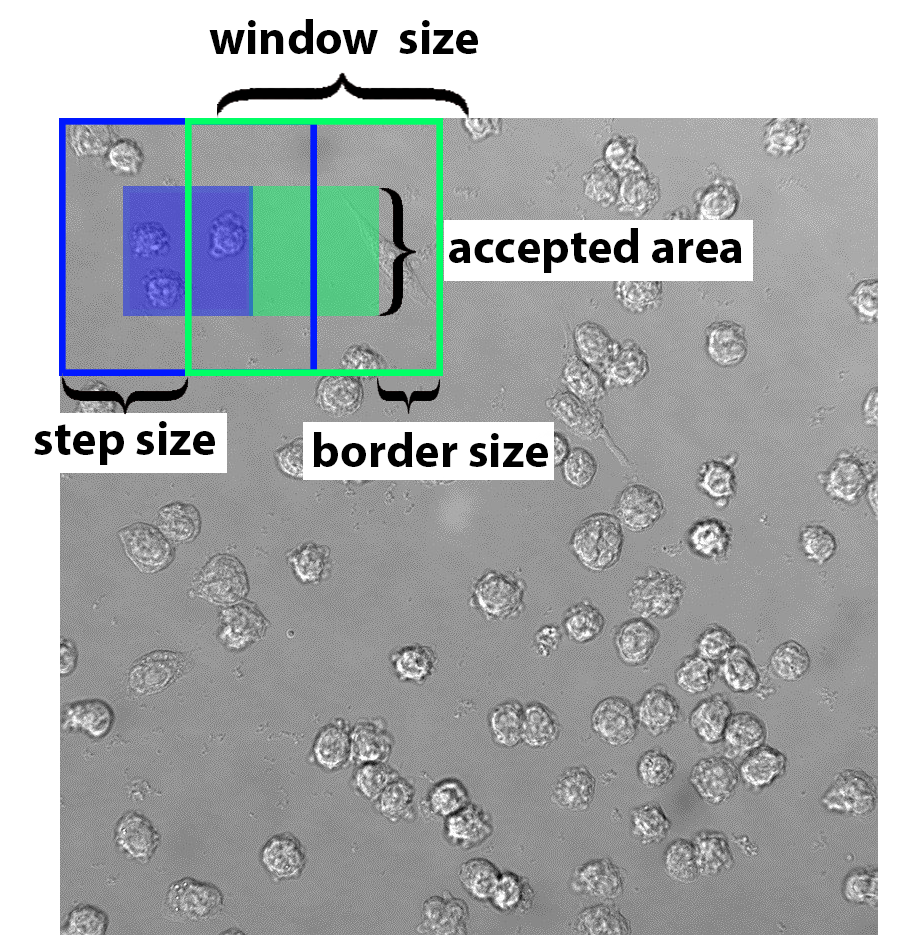
\includegraphics[width=0.3\linewidth]{bilder/sliding-window.png}
		\caption{Sliding window approach for fluorescence prediction}\label{fig:sliding-window}
	\end{center}
\end{figure}
The reason why the full prediction is not accepted to form the output lies in the following: trained models are less accurate on the borders of the crops rather than in the center. Most of the times there are cells on the borders of the crops that were sliced and therefore it might be impossible to make a good prediction for them just due to the lack of input information. Therefore, the step size has to be smaller than the window size, so that the windows are overlapping and for each prediction we use only the image center and are allowed to ignore predictions on the border (see the comparison between different border sizes in Figure \ref{fig:crops-combination}). This is discussed in more detail in Section [TODO reference the section]. Such an approach helps to reduce the effect of grid visibility on the image composed of many small crops. This can be seen in the left part of Figure 5 as opposed to the non-visible borders in the same Figure on the right. This would of course take more time to created the predictions, however, the speed is less crucial in comparison to the accuracy of the predictions.

\begin{figure}[htb]
	\begin{center}
		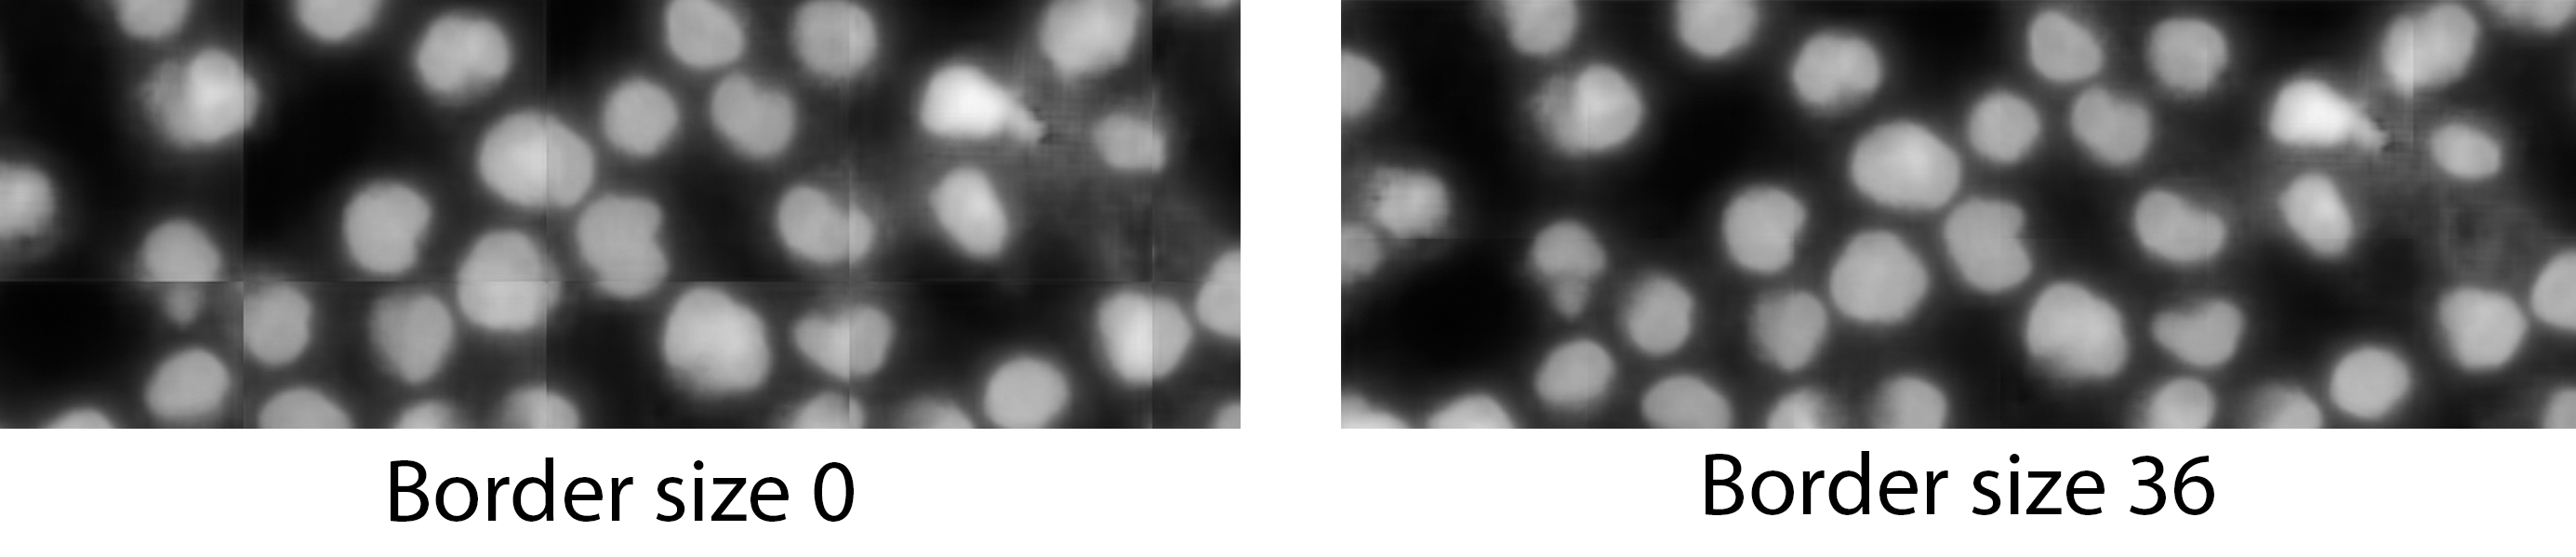
\includegraphics[width=\linewidth]{bilder/crops_combination/crops-combination.png}
		\caption{Difference of overlap between predictions on the resulting image}\label{fig:crops-combination}
	\end{center}
\end{figure}